\documentclass[10pt]{beamer}

\usetheme{CambridgeUS}
\usepackage[english, russian]{babel}
\usepackage[utf8]{inputenc}
\usepackage{caption}
\usepackage{minted}
\usepackage{etoolbox}
\usepackage{multicol}
\AtBeginEnvironment{minted}{\singlespacing%
    \fontsize{10}{10}\selectfont}

\title[\href{https://goo.gl/NRgp8K}{https://goo.gl/NRgp8K} (Term 1)]{Введение в программирование}
\author[Гусев Илья, Булгаков Илья]{Гусев Илья, Булгаков Илья}
\institute[МФТИ] 
{Московский физико-технический институт\\*}
\date{Москва, 2018}
\subject{Computer Science}

\begin{document}

\begin{frame}
  \titlepage
\end{frame}

\begin{frame}{Содержание}
\tableofcontents
\end{frame}

\section{Введение}

\subsection{Преподаватели}

\begin{frame}{Преподаватели: Илья Булгаков}
\textbf{Илья Булгаков}:
\begin{itemize}
    \item 
\end{itemize}
\end{frame}

\begin{frame}{Преподаватели: Илья Гусев}
\textbf{Илья Гусев}:
\begin{itemize}
    \item Выпускник ФИВТ МФТИ (бакалавриат в 2016, магистратура в 2018)
    \item Аспирант на кафедре компьютерной лингвистики МФТИ
    \item Преподаватель кафедры алгоритмов и технологий программирования (АТП) с 2016 года, кафедры компьюетрной лингвистики с 2017 года.
    \item Бэкенд-разработчик в ABBYY LingvoLive в 2016-2017 годах, десктоп-разработчик в группе разработки инструментов машинного обучения в ABBYY в 2017-2018 годах, инженер в области машинного обучения в группе качества Яндекс.Новостей с 2018 года по настоящее время
    \item Профессиональные интересы: глубокое обучение (deep learning) и обработка естественных языков (NLP)
    \item \href{https://github.com/IlyaGusev/}{https://github.com/IlyaGusev/}
\end{itemize}
\end{frame}

\subsection{Структура курса}
\begin{frame}[fragile]{Структура курса}
\begin{enumerate}
\item Алгоритмы:
    \begin {itemize}
        \item 3 семестра
        \item Экзамены в 1 и 3
        \item 1 ак. час лекций в неделю
    \end {itemize}
\item C++:
    \begin {itemize}
        \item 2 семестра
        \item Экзамен во 2
        \item 1 ак. час лекций в неделю
    \end {itemize}
\item Практика
    \begin {itemize}
        \item 3 семестра,
        \item Во всех зачёты
        \item 2 ак. часа семинаров в неделю
    \end {itemize}
\end{enumerate}
Итого: 3 экзамена, 3 зачёта, 4 ак. часа в неделю на протяжении 3 семестров
\end{frame}


\subsection{Правила зачёта}
\begin{frame}[fragile]{Правила зачёта}{Оценки}
\begin{itemize}
\item 1 модуль - 25 балла
\item 2 модуль - 25 балла
\item 3 модуль - 25 балла
\item 4 модуль - 25 балла
\item 20 баллов за задачи и 5 баллов за ответ на контрольной
\item Сроки сдачи ограничены для каждого модуля
\item Критерий приёма задачи: Яндекс.Контест + review кода
\item Review кода = style + правильность алгоритма + функциональная декомпозиция
\end{itemize}
\end{frame}


\begin{frame}[fragile]{Правила зачёта}{Оценки}
\begin{itemize}
\item 0-39 баллов - 1 (неуд)
\item 40-49 баллов - 2 (неуд)
\item 50-56 баллов - 3 (удовл)
\item 57-65 баллов - 4 (удовл)
\item 66-71 баллов - 5 (хор)
\item 72-77 балла - 6 (хор)
\item 78-83 баллов - 7 (хор)
\item 84-88 баллов - 8 (отл)
\item 89-93 балла - 9 (отл)
\item 94-100 баллов - 10 (отл)
\end{itemize}
\end{frame}

\begin{frame}[fragile]{Правила зачёта}{Посещаемость, списывание}
\begin{itemize}
\item Про посещаемость: она напрямую не влияет на оценку
\item Про списывание: любое дублирование чужого кода штрафуется -5 и незачётом по задаче
\end{itemize}
\end{frame}

\begin{frame}[fragile]{Правила зачёта}{Кодстайл}
\begin{itemize}
\item Понятные названия переменных (однобуквенные только как счётчики в циклах или заданные в условии задачи)
\item Не должно быть утечек памяти
\item Грамтоная декомпозиция на функции. В main должен находиться ввод данных, вызов функции, которая решает задачу, вывод результата. Ввод/вывод производится только в main, решение - только в отдельном наборе функций
\item Переменные должны объявляться по месту использования (уже давно >= С99)
\item Глобальными переменными пользоваться нельзя
\item Остальное: \href{https://goo.gl/Ztu6td}{https://goo.gl/Ztu6td}
\end{itemize}
\end{frame}

\section{Языки программирования}
\subsection{Языки программирования}
\begin{frame}{Компьютер}
\begin{center}

\includegraphics[width=6cm, height=7cm]{Term_1/Source/Pirctures/not_good.jpg}
\end{center}
\end{frame}

\begin{frame}{Компьютер}
\begin{enumerate}
    \item Железо
    \item Драйверы
    \item Операционная система
    \item Языки программирования и библиотеки программ
    \item Пользовательские программы
\end{enumerate}
\end{frame}

\begin{frame}{Языки программирования}
Компьютер:
\begin{enumerate}
    \item Не понимает человеческих команд и желаний
    \item Оперирует 1 и 0
    \item Может складывать/вычитать/умножать числа, считывать данные из ячейки памяти и записывать их в ячейку памяти
    \item Архитектура фон Неймана
\end{enumerate}

Язык программирования - прослойка между желаниями человека и компьютером
\end{frame}

\begin{frame}{Языки программирования}
\begin{itemize}
    \item 'Старые': Lisp, Cobol, Fortran, Basic, Pascal, Ada, ...
    \item Основные: C, C++, Java, Python, C\#, Javascript, PHP, ...
    \item Молодые: Go, Rust, Swift, Kotlin, Scala, ...
    \item Нишевые: Haskell, Clojure, Erlang, D, F\#, ...
    \item Эзотерические: Brainfuck, Whitespace, Shakespeare, FiM++, ...
\end{itemize}
\end{frame}

\subsection{Почему C++?}
\begin{frame}{Почему C++?}
\begin{enumerate}
    \item Универсальность: компиляторы под любую платформу
    \item Сообщество: широкая поддержка, новые стандарты, отличные книжки и документация, поддержка в IDE
    \item Низкоуровневость: ручное управление памятью по умолчанию, скорость исполнения
    \item Сложность: если выучили C++, то остальное будет легко
    \item Популярный синтаксис: Java, C#, Javascript имеют Си-подобный синтаксис
    \item Востребованность: огромное наследие; использование в больших корпорациях; языки операционных систем и драйверов; в ближайшие 5-10 лет точно актуальны
\end{enumerate}
\end{frame}

\begin{frame}{Почему НЕ C++?}
\begin{enumerate}
    \item "Так исторически сложилось": много решений в дизайне языков принимались впервые и иногда неправильно; много противоречивых концепций 
    \item Перегруженный синтаксис: во многих языках программы будут в 2-100 раз короче; в "Hello world!" на С++ есть МНОГО непонятных вещей
    \item Отсутствие менеджера пакетов: сложно подключать внешние библиотеки, а значит сложно сделать что-то прикладное
\end{enumerate}

Замены C++: C\#, Rust, Go
\end{frame}

\begin{frame}{Профессии}
Алгоритмы нужны любому разработчику, любому аналитику и любому менеджеру в IT. \\
\\
C необходим:
\begin{enumerate}
    \item Разработчику встраиваемых систем
    \item Системному инженеру
\end{enumerate}

С++ необходим:
\begin{enumerate}
    \item Десктоп-разработчику
    \item Разработчику распределённых систем
    \item Разработчику игр
\end{enumerate}

C++ может пригодится:
\begin{enumerate}
    \item Бэкенд-разработчику
    \item Мобильному разработчику
\end{enumerate}
\end{frame}

\begin{frame}[fragile]{Зарплаты}
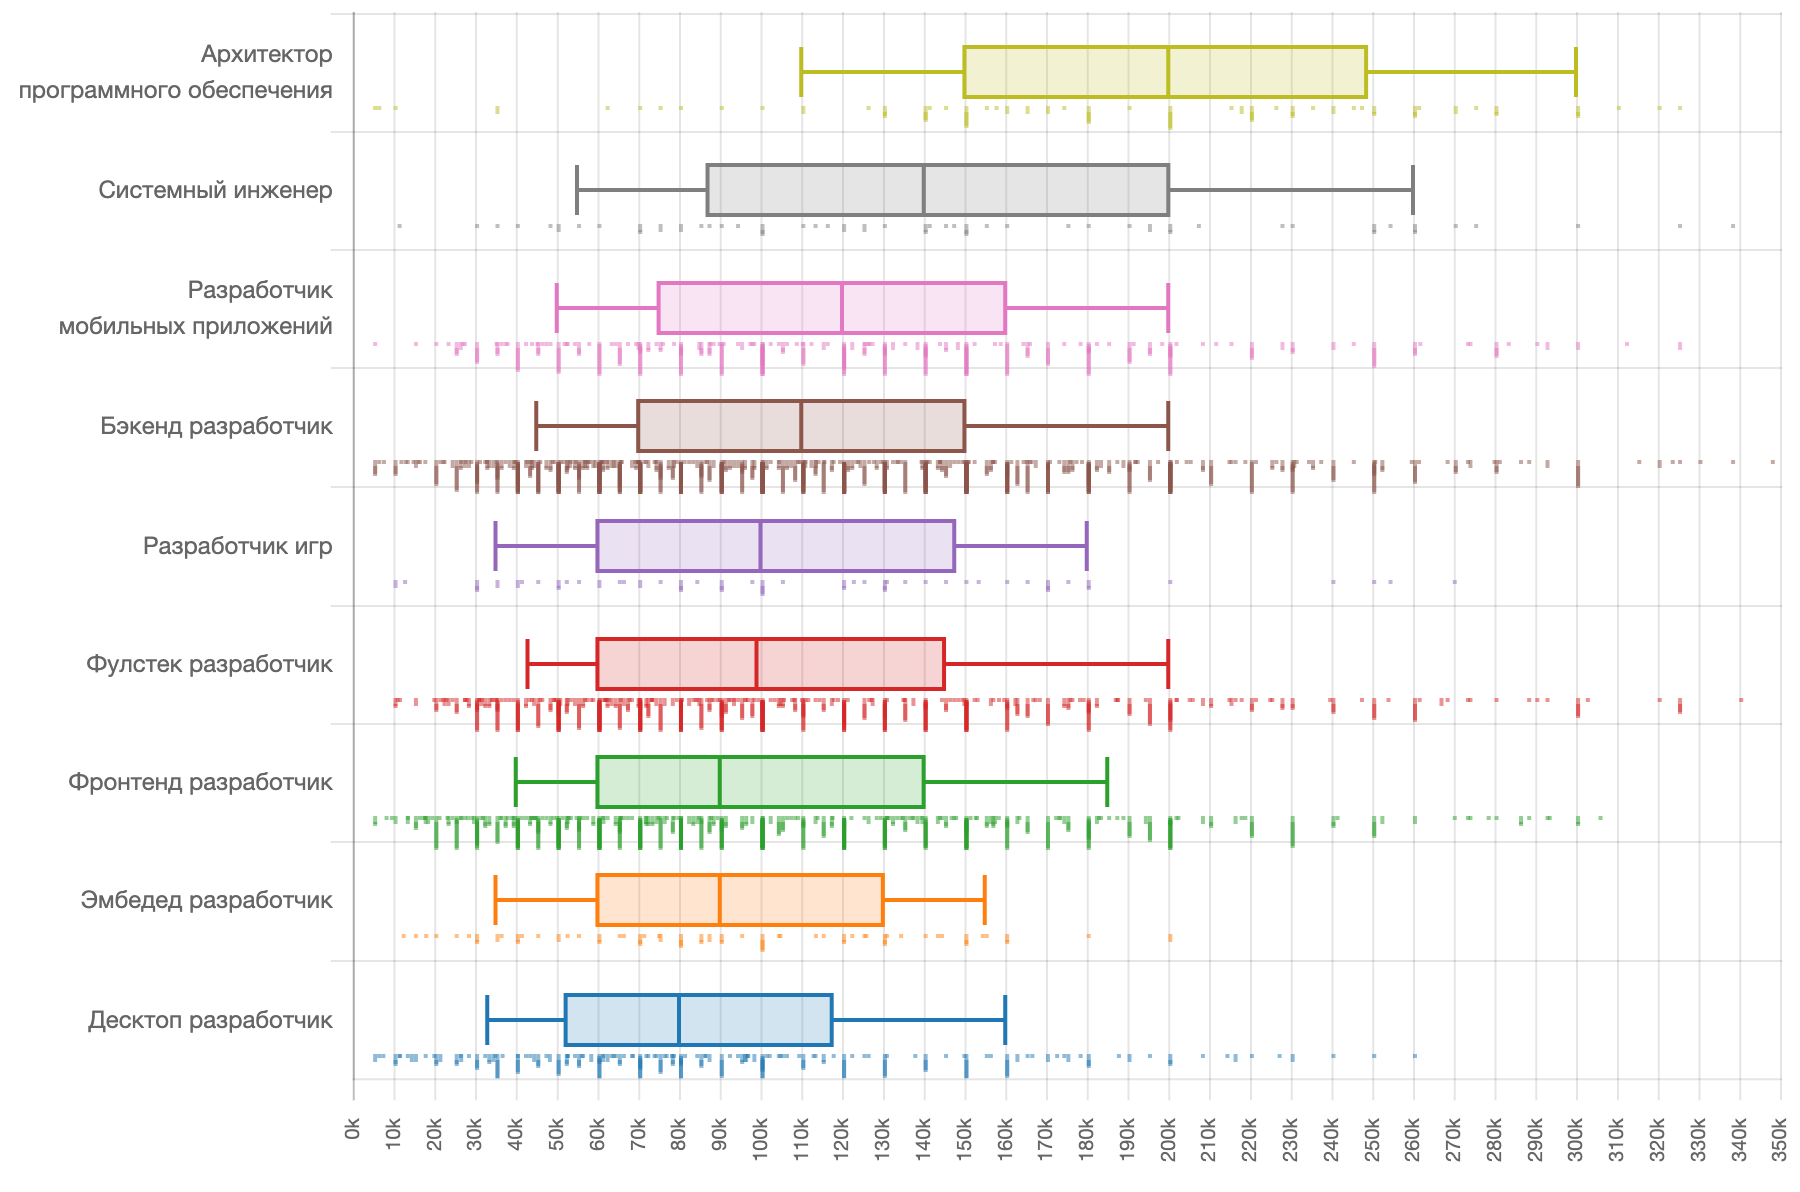
\includegraphics[width=10cm, height=7cm]{Term_1/Source/Pirctures/salaries.png}\\
\href{https://habr.com/ru/company/moikrug/blog/461855/}{https://habr.com/ru/company/moikrug/blog/461855/}
\end{frame}


\section{Язык Си}
\subsection{Свойства языка}
\begin{frame}[fragile]{Свойства языка}
\begin{itemize}
    \item Компилируемый
    \item Процедурный
    \item Статически типизируемый
    \item Возможность модификации памяти через указатели
\end{itemize}
\end{frame}

\begin{frame}[fragile]{Компилируемость}
\begin{multicols}{2}
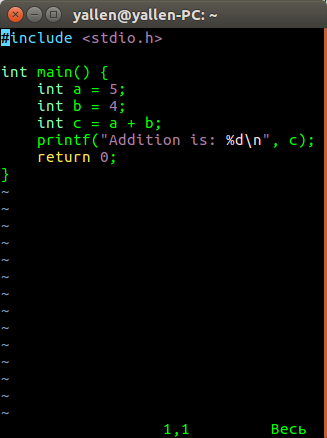
\includegraphics[width=5cm, height=7cm]{Term_1/Source/Pirctures/c-example.png}
\vfill\eject
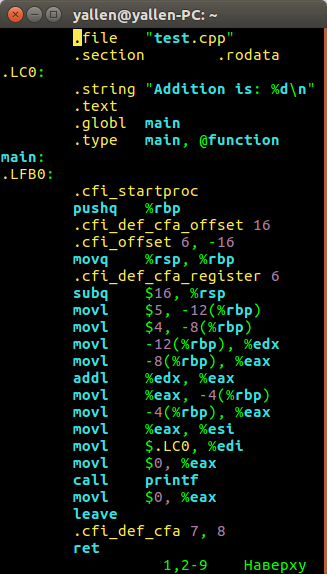
\includegraphics[width=4cm, height=7cm]{Term_1/Source/Pirctures/assembler-example.png}
\end{multicols}
\end{frame}

\begin{frame}[fragile]{Указатели}
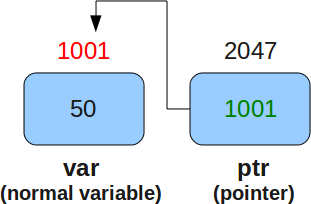
\includegraphics[width=8cm, height=5cm]{Term_1/Source/Pirctures/c-var-ptr.png}
\end{frame}

\subsection{IDE}
\begin{frame}[fragile]{IDE}
F
\end{frame}

\appendix
\section<presentation>*{\appendixname}
\subsection<presentation>*{Useful links}

\begin{frame}[allowframebreaks]
  \frametitle<presentation>{Полезные ссылки}
    
  \begin{thebibliography}{10}
{
  \beamertemplatebookbibitems
  % Start with overview books.
  \bibitem{Kormen1}
  \texttt{Т.Кормен, Ч.Лейзерсон, Р.Ривест, К.Штайн - Алгоритмы. Построение и анализ. - 2013, djvu}
  \newblock \href{https://bit.ly/2wFzphU}{\texttt{https://bit.ly/2wFzphU}}
  
  \bibitem{Kormen2}
  \texttt{Т.Кормен, Ч.Лейзерсон, Р.Ривест, К.Штайн - Алгоритмы. Построение и анализ. - 2013, pdf}
  \newblock \href{https://bit.ly/2PpdqUc}{\texttt{https://bit.ly/2PpdqUc}}
  
  \bibitem{CKR}
  \texttt{Б.Керниган, Д.Ритчи - Язык программирования C - 2009, djvu}
  \newblock \href{https://bit.ly/2PwcVb8}{\texttt{https://bit.ly/2PwcVb8}}
  
  \bibitem{Lippman}
  \texttt{С.Липпман, Ж.Лажойе - Язык программирования C++. Базовый курс. - 2014, djvu}
  \newblock \href{https://bit.ly/2LQhk6z}{\texttt{https://bit.ly/2LQhk6z}}
  
  \bibitem{std}
  \texttt{Working Draft, Standard for Programming Language C++}
  \newblock \href{https://bit.ly/2PvGSIb}{\texttt{https://bit.ly/2PvGSIb}}
  
  \beamertemplatearticlebibitems
  
  \bibitem{wiki}
  \texttt{Викиконспекты}
  \newblock \href{http://neerc.ifmo.ru/wiki/}{\texttt{http://neerc.ifmo.ru/wiki/}}
  
  \bibitem{cppreference}
  \texttt{Справка по C++}
  \newblock \href{https://ru.cppreference.com/w/}{\texttt{https://ru.cppreference.com/w/}}
  
  \bibitem{superfaq}
  \texttt{C++ Super-FAQ}
  \newblock \href{https://isocpp.org/faq}{\texttt{https://isocpp.org/faq}}
   
  \bibitem{StackOverflow}
  \texttt{StackOverflow}
  \newblock \href{https://stackoverflow.com/}{\texttt{https://stackoverflow.com/}}
  
  \bibitem{Хабр}
  \texttt{Хабр}
  \newblock \href{https://habr.com/}{\texttt{https://habr.com/}}
  
  \bibitem{Хабр: Зарплаты в ИТ в первом полугодии 2019 года}
  \texttt{Хабр: Зарплаты в ИТ в первом полугодии 2019 года}
  \newblock \href{https://habr.com/ru/company/moikrug/blog/461855/}{\texttt{https://habr.com/ru/company/moikrug/blog/461855/}}
  
  \bibitem{Исследования Яндекса - Обзор рынка ИТ-вакансий}
  \texttt{Исследования Яндекса - Обзор рынка ИТ-вакансий}
  \newblock \href{https://yandex.ru/company/researches/2019/it-jobs}{\texttt{https://yandex.ru/company/researches/2019/it-jobs}}
  
  \bibitem{StackOverflow: Developer Survey Results
2018}
  \texttt{StackOverflow: Developer Survey Results
2018}
  \newblock \href{https://insights.stackoverflow.com/survey/2018}{\texttt{https://insights.stackoverflow.com/survey/2018}}
  
  \bibitem{Хабр: Преимущества C++ как первого языка для обучения программированию}
  \texttt{Хабр: Преимущества C++ как первого языка для обучения программированию}
  \newblock \href{https://habr.com/ru/post/202466/}{\texttt{https://habr.com/ru/post/202466/}}
  
  \bibitem{Хабр: Ликбез по типизации в языках программирования}
  \texttt{Хабр: Ликбез по типизации в языках программирования}
  \newblock \href{https://habr.com/ru/post/161205/}{\texttt{https://habr.com/ru/post/161205/}}
  
  \bibitem{Career levels across companies}
  \texttt{Career levels across companies}
  \newblock \href{https://www.levels.fyi/}{\texttt{https://www.levels.fyi/}}

}


  \end{thebibliography}
\end{frame}

\end{document}


